\documentclass[MathsNotesBase.tex]{subfiles}

\date{\vspace{-6ex}}


\begin{document}
	\chapter*{Code Examples}
	
	\subsection{Inline maths}
	${}$ % atomic maths
	${\bm{}}$ % atomic bold maths
	
	\subsection{Maths bold font}
	$\bm{x} = 2$
	
	\subsection{Align section with iff and sidecomments}
	\begin{align*}
		&& a \in ker \; \phi \iff \phi(a) &= 1 \\
		&\implies & \phi(ba\inv{a}) &= \phi(a) \cdot 1 \cdot \phi(\inv{a}) \\
		&\iff & \phi(ba\inv{a}) &= \phi(a)\inv{\phi(a)} &\sidecomment{using \autoref{prop:isomorphism_preserves_structure}} \\
		&\iff & \phi(ba\inv{a}) &= 1.
	\end{align*}	
%	\begin{align*}
%		&&  &=  \\
%		&\iff &  &=  &\sidecomment{} \\
%	\end{align*}

	\subsection{Propositions and Theorems}
	\labeledProposition{}{}
	\begin{proof}
	\end{proof}
	
	\subsection{Inline image}
	\begin{figure}[h!]
		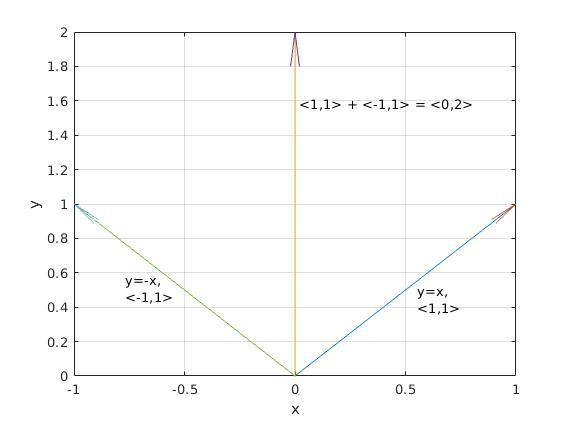
\includegraphics[width=\linewidth]{resources/img/not_closed_under_addition.png}
		\caption{The blue arrows are vectors whose scalar multiples will all be in the same line as the blue arrows but the red arrow shows what happens if we add them; the result lies outside of both lines.}
	\end{figure}
	
	\subsection{Tables}
	\begin{table}[h!]%
		\caption{Maximum load and nominal tension.}
		\label{aggiungi}\centering%
		\begin{tabular}{clccc}
			\toprule%
			$D$ & & $P_u$ & $\sigma_N$ \\
			(in)& &(lbs) & (psi) \\ \toprule%
			5 & test 1 & 285 & 38.00 \\
			& test 2 & 287 & 38.27 \\
			& test 3 & 230 & 30.67 \\ \midrule
			10 & test 1 & 430 & 28.67 \\
			& test 2 & 433 & 28.87 \\
			& test 3 & 431 & 28.73 \\ \bottomrule
		\end{tabular}
	\end{table}
	
	\begin{tabular}[h!]{*4c}
		& &\multicolumn{2}{c}{$p_{2}$}\\
		& & $F$ &$D$ \\\cline{3-4}
		\multirow{2}{*}{$p_{1}$}& $F$ & \multicolumn{1}{|c|}{($1-C$,$1-C$)} & \multicolumn{1}{c|}{($-C,1$)} \\\cline{3-4}
		& $D$ & \multicolumn{1}{|c|}{($-1,C$)} &\multicolumn{1}{c|}{($0,0$)}\\\cline{3-4}
	\end{tabular}
	\subparagraph{$S_3$}
	
	\subsection{Boxed text}
	\noindent\fbox{%
		\parbox{\textwidth}{%
			Every group, at a minimum, has two trivial subgroups: the maximal subgroup - the group itself; and the minimal subgroup - the set containing just the identity. A subgroup that is neither of these is known as a \mbox{\textit{proper subgroup}}.
		}%
	}\bigskip

	\subsection{Less-than page width align section}
	\[\begin{array}{*6c}
	&1 &&\longmapsto &&1 \\
	&x &&\longmapsto &&x^2 \\
	&x^2 &&\longmapsto &&x \\
	\end{array}\]
	
	\subsection{Numbered Referrable Examples}
	\begin{exe}
		\ex Wh/Quantifier Interactions\label{WHQ}
		\begin{xlist}
			\ex[]{What did everyone bring to the party?}
			\begin{xlist}
				\ex {Beer. \hfill \emph{Individual answer}} \label{beer_example}
				\ex {Bill brought beer, Sue brought wine, Sam brought vodka \hfill \emph{Pair List answer}}
				\ex {His favourite drink. \hfill \emph{Functional answer}}
				\exr {beer_example}
			\end{xlist}
		\end{xlist}
	\end{exe}
	As we can see in (\ref{WHQ}) there is a subject/object asymmetry in the availability of the Pair list and functional answers. Also \ref{beer_example} is somehow relevant.
	\subsubsection{Single-level examples list}
	\begin{exe}
		\ex {	Let $C = \{ a^{n-1}, \cdots, a^{-2}, a^{-1}, 1, a, a^2, \cdots, a^{n-1} \}$ be a finite cyclic group. Then the map,
			\[ \phi : \Z{+} \longmapsto C \; \suchthat \; \phi(n) = a^n \]
			is a homomorphism. Note that if $C$ were an infinite cyclic group then this would be an isomorphism. }\label{ex_infinite_cyclic_group}
		\ex {the sign of a permutation $ sign : S_n \longmapsto {\pm1} $}\label{ex_sign_permutation}
		\ex {the determinant function $ det : GL_n(\R{}) \longmapsto \R{\times} $}\label{ex_determinant}
		\ex {an arguably trivial example is called the \textit{inclusion} map $i : H \longmapsto G$ of a subgroup $H$ into a group $G$, defined by $i(x) = x$. It functions as the identity for elements in the subgroup $H$ but, since it is not surjective, there is no inverse mapping.}\label{ex_inclusion_map}
	\end{exe}

	\subsection{Code listings}
	\lstinputlisting[language=Python]{./resources/code/python/converge_to_minus_2.py}
	
	\subsection{Text block with background color}
	\begin{tcolorbox}[enhanced jigsaw,colback=note_bg,boxrule=0pt,arc=0pt]
		\begin{itemize}
			\item Item 1
			\item Item 2
			\item Item 3
		\end{itemize}
	\end{tcolorbox}
	
\end{document}
